\documentclass[a4paper,man,natbib]{apa6}

\usepackage[english]{babel}
\usepackage[utf8x]{inputenc}
\usepackage{amsmath}
\usepackage{graphicx}
\usepackage[colorinlistoftodos]{todonotes}

\title{Gender Attrition in Computer Science: An Investigation of Why Female Students Report Under-Performing in Introductory Courses}
\shorttitle{gender attrition in computer science}
\author{Benjamin Floyd}
\affiliation{University of Virginia}

%\abstract{Your abstract here.}

\begin{document}
\maketitle

\section{Introduction}
\label{sec:intro}
In the field of Computer Science (CS), gender disparity has been a challenge
for over 40 years~\citep{Dale-studentprofile, Camp, Cohoon-retention,
Frenkel-women, Klawe-increasingpaarticipation, Montanelli-women,
Spertus-whysofew}. Specifically, women are typically underrepresented in the
field. Today, the number of women in undergraduate Computer Science programs
hovers around 18\%, nationally~\citep{womenincs-DOE}. Computer Science departments
traditionally have trouble recruiting female students; this naturally accounts
for some of the gender disparity. However, departments also suffer from
attrition of female students once they enter the major. A reason commonly cited
among females who decide to leave the major is that they under-perform in
introductory classes. Loosely, this claim admits two broad possibilities:
either female students actually under-perform in introductory CS courses, or they
only perceive that they under-perform. This paper considers each of these
possibilities in turn. First, we investigate if female students actually
perform worse than their male peers in introductory classes. We conclude that
there is no evidence to support the claim that females under-perform in this
regard. Second, we investigate if females only perceive that they are
under-performing and consider possible causes of this perception. To explore
these questions, we analyze survey and grade data for over one thousand
students across introductory CS courses.

\section{Methods}
\label{sec:methods}
To address the research questions, we analyze two sources of data: anonymous
surveys, and student grade information. 

\subsection{Surveys}
\label{sec:survey}
Students answered an IRB approved, web-based survey with approximately ten
questions. The survey included demographic questions, Likert-scale questions,
and free-form questions. The surveys were distributed at various points such as the
beginning of a course, the end of a course, or when dropping a class. Students
were tracked through an anonymous identifier in order to recognize when the
same student took the survey more than once. The dataset contains responses
from 1019 distinct undergraduate students who were enrolled in Computer Science
introductory courses between 2008 and 2010 at the University of Virginia.

\subsection{Grades}
\label{sec:grade}
Instructors provided final grade and gender data for 1,023 distinct
undergraduates who were enrolled in CS1 or CS2 courses between 2008 and 2010 at
the University of Virginia. This amounted to a total of 2,021 final grade
instances. Student genders were manually labelled as male, female, or unknown
based on name and photograph information. Letter grades were converted to the
standard College Board GPA scale (i.e. "B"=3.0, "B+"=3.3, etc.). Final grades
marked as either "incomplete" or "pass/fail" were omitted from the dataset (41
out of 2062 were not included). Table~\ref{tab:courses} shows the classes involved in
the creation of this dataset, as well as the sample sizes for each year. The
University of Virginia CS Department features two different CS1 classes based
on intended degree; additionally, the CS2 class is considered introductory. 

Because of the anonymous nature of the surveys, it was impossible to link a
particular survey respondent to a set of CS course grades.

\section{Results}
\label{sec:results}
We address two primary research questions by analyzing the dataset described in
the Methods section. These questions correspond to two broad explanations for
why female students report under-performing in introductory CS courses. First,
we evaluate whether female students actually perform worse that their male peers
in these courses; we find no evidence to support the claim that females perform
worse than males in this regard. Then, we investigate if females only perceive
that they are under-performing, and discuss possible factors that contribute to
this perception. 

\subsection{RQ1: Do females under-perform their male peers in introductory CS
classes?} We use final grade data to address this question. These data are
converted into a numerical GPA scale, and are partitioned by gender (male,
female, and unknown). The descriptive statistics for these data are located in
Table~\ref{tab:descriptive}. Additionally, Figure~\ref{fig:boxplot} shows a
boxplot of the grade data, split by gender group. To investigate the
differences in final grade based on gender, we performed an ANOVA with $\alpha
= .05$. The ANOVA did not yield a significant effect of gender on final grade,
$F(2,2018)=2.396$, $p=.0914$, $\omega^2=.0014$. This indicates that grades do
not differ by gender group. However, since we were most interested in the
differences between males and females, we also conducted a two-sided
independent samples $t$-test using grade data from only those groups (i.e. the
unknown group was dropped for this test). This $t$-test, performed at
$\alpha=.05$, did not reveal any significant difference between males' and
females' final grades, $t(1615)=1.8435$, $p=.0656$, $d=.0999$. The 95\%
confidence interval for male$-$female is [-.0061,.1943]. This confirms our
findings from the ANOVA: grade data does not differ significantly by gender.

\subsection{RQ2: Do females perceive themselves as under-performing?}
Since there is no significant difference between the actual performance of
males and females in introductory CS courses, the remaining broad explanation
for females reporting under-performance is that they only perceive the
discrepancy. We investigate this hypothesis by analyzing the survey data. In
particular, we focus on two questions: (1) "I am doing well in the CS/CPE
program based on my own expectations" and (2) "I am doing well in the CS/CPE
program based on the expectations of others". Students answered these questions
on a 5-point Likert scale ranging from "Strongly Disagree" to "Strongly Agree".
The response frequencies, partitioned by gender, are in
Table~\ref{tab:expec-own} and Table~\ref{tab:expec-other}, respectively. 

A chi-square test of independence was performed for each of these questions to
investigate the relationship between gender and survey responses. The test for
"I am doing well \dots based on my own expectations" did not reveal a
significant effect on responses by gender at $\alpha=.05$, $\chi^2(4)=7.509$,
$p=.1113$, $V=.1554$. However, a chi-square test for "I am doing well \dots
based on the expectations of others" was significant at $\alpha=.05$,
$\chi^2(4)=12.0696$, $p=.0168$, $V=.1964$. This means that gender significantly
affects the response distrobution to this question. Computing the standardized
residuals reveals that both the "Strongly Agree" and "Strongly Disagree"
options had significant differences. 

\section{Discussion}
Female students report that they under-perform in introductory CS courses
compared to their male peers. In this paper, we propose and evaluate two
possible explanations. First, we investigate whether female students actually
perform worse than male students by analyzing final grade data. We perform an
ANOVA to test for differences in grade data based on all three gender groups
(male, female, and unknown). The ANOVA did not provide statistically
significant results. We also conducted a two-sided independent samples $t$-test
based only on the grade data of the two groups of interest (males and females).
This, too, failed to provide significant evidence that gender affects final
grade in introductory courses. The p-value for this test was surprisingly low;
the results could be considered marginally significant. However, the effect
size for this test was also very small, signifying that, even if the difference
between males and females was statistically significant, it was only about 10\%
of a standard deviation.

Since females do not under-perform males in a significant manner, we
investigate the possibilty that female students only perceive that they perform
poorly in these courses. We use two survey questions to address this
hypothesis. The first question asks for a Likert-style response to the
following claim: "I am doing well in the CS/CPE program based on my own
expectations". We perform a chi square test of independence to determine if
gender affects response; the test did not reveal a significant difference.
However, we also perform a chi square test of independence on reponses to "I am
doing well in the CS/CPE program based on the expectations of others". This
test showed that gender affects response to this question in a statistically
significant way. The analysis of these survey results provides insight into the
source of the perception of under-performance in female students. One
possibility is that female students have higher expectations of themselves, and
thus are more prone to perceiving poor performance. However, the first chi
square test reveals that this is not the case: females and males have no
significant difference in their own expectations. Another possibility is that
female students perceive that others have higher expectations of them than male
students do. The second chi square test supports this claim with statistical
significance. This indicates that female students perceive that others expect more of
them, and thus the females are more likely to report under-performing.

\begin{table}
\begin{tabular}{l|l|l}
Course ID	& Semesters						& Students \\\hline
CS1 (BS)	& F'08, S'09, F'09, F'10, S'10	& 1320 \\
CS1 (BA)	& S'09, F'10, S'10				& 172 \\
CS2			& F'08, F'09, S'09, S'10		& 570
\end{tabular}
\caption{\label{tab:courses}Courses studied in final grade data. F/S indicates Fall or Spring semester.}
\end{table}

\begin{table}
\begin{tabular}{l|c|c|c}
		& male	& female	& unknown \\\hline
N		& 1100	& 517		& 404 \\
Mean	& 3.25	& 3.15		& 3.16 \\
sd		& 0.93	& 0.97		& 0.99
\end{tabular}
\caption{\label{tab:descriptive}Descriptive statistics for final grade data.}
\end{table}

\begin{figure}
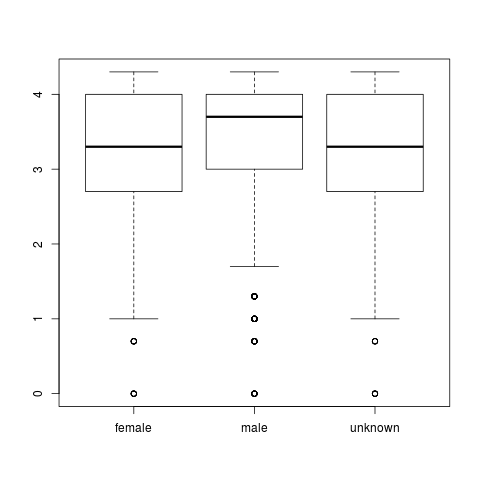
\includegraphics[width=0.5\textwidth]{boxplot.png}
\caption{\label{fig:boxplot}A boxplot of grade data, split by gender group.}
\end{figure}

\begin{table}
\begin{tabular}{l|l|l|l|l|l}
		& Strongly Agree	& Agree	& Neutral	& Disagree	& Strongly Disagree \\\hline
males	& 29				& 68	& 39		& 36		& 11 \\
females & 9					& 51	& 33		& 22		& 13
\end{tabular}
\caption{\label{tab:expec-own}Frequencies of responses to "I am doing well in the CS/CPE program based on my own expectations".}
\end{table}

\begin{table}
\begin{tabular}{l|l|l|l|l|l}
		& Strongly Agree	& Agree	& Neutral	& Disagree	& Strongly Disagree \\\hline
males	& 34				& 64	& 55		& 25		& 6 \\
females & 10				& 41	& 50		& 17		& 11 
\end{tabular}
\caption{\label{tab:expec-other}Frequencies of responses to "I am doing well in the CS/CPE program based on the expectations of others".}
\end{table}

\bibliography{my-bib}

\end{document}

%
% Please see the package documentation for more information
% on the APA6 document class:
%
% http://www.ctan.org/pkg/apa6
%
